% % no answer key
% \documentclass[letterpaper]{exam}

% answer key
\documentclass[letterpaper, landscape]{exam}
\usepackage{2in1, lscape} 
\printanswers{}

\usepackage{units} 
\usepackage{parskip} 
\usepackage{xfrac} 
\usepackage[fleqn]{amsmath}
\usepackage{cancel}
\usepackage{float}
\usepackage{mdwlist}
\usepackage{booktabs}
\usepackage{cancel}
\usepackage{polynom}
\usepackage{caption}
\usepackage{fullpage}
\usepackage{comment}
\usepackage{enumerate}
\usepackage{graphicx}
\usepackage{mathtools} 
\usepackage{commath}
\usepackage[group-separator={,}]{siunitx}

\everymath{\displaystyle}

\title{Statistics \\ Chapter 14 Homework}
\date{\today}
\author{}

\begin{document}

  \maketitle

  \section{Homework}
  Chapter 14: 34, 36--38, 40, 42--46, 48--53, 55, 57

  \ifprintanswers{}
    \section{Solutions}
    \begin{description}

      \item[34] 
        \begin{enumerate}[(a)]
          \item 
            \[
              137 \pm 2.576 \cdot \frac{65}{\sqrt{269}} \approx 137 \pm 10.2
            \]
            The 99\% confidence interval is from \fbox{126.8 to 147.2}.

          \item The students selected must be a simple random sample.

        \end{enumerate}

      \item[36] 
          \[
            248 \pm 2.576 \cdot \frac{65}{\sqrt{269}} \approx 248 \pm 10.2
          \]
          The 99\% confidence interval is from \fbox{237.8 to 258.2}.

      \item[37] This is incorrect. The statement should be about the population
        mean ($\mu$), not any particular individual.

        It's possible that nobody in the population has a BMI in the range
        described. For example, a population with BMIs of 
        
        \{ 25, 25, 25, 29, 29, 29 \} 
        
        has $\mu = 27$ but nobody with a BMI between 26.2 and 27.4.

        For both problems 37 and 38, the correct statement is: ``We can be 95\%
        confident that the population mean is between 26.2 and 27.4.''

      \item[38] This is incorrect. The statement should be about the population
        mean ($\mu$), not future sample means ($\bar{x}$). 

        If the population mean happens to be towards one or the other end of
        this range, many similar samples will be outside of the range. For
        example, if $\mu$ is actually 27.3, about have of $\bar{x}$ from other
        samples will be outside of the 26.2 to 27.4 range.

      \item[40]
        \begin{enumerate}[(a)]
          \item 
            \noindent
            \begin{itemize*}
              \item $H_0$: $\mu = 120$
              \item $H_a$: $\mu > 120$
            \end{itemize*}

          \item
            \begin{align*}
              \sigma_{\bar{x}} &= \frac{64}{\sqrt{269}} = 3.902 \\
              z                &= \frac{137 - 120}{3.902} \approx \boxed{ 4.36 }
            \end{align*}

          \item The p-value is 
            \[
              p \approx = \boxed{ 0.0005 } 
            \]
            There is 0.05\% chance of observing a survey result of 137 if
            students actually study 120 minutes or less per night, so we can
            conclude they probably study more than 120 minutes per night.

        \end{enumerate}

      \newpage

      \item[42]
        \begin{enumerate}[(a)]
          \item 
            \noindent
            \begin{itemize*}
              \item $H_0$: $\mu = 5.19$
              \item $H_a$: $\mu \ne 5.19$
            \end{itemize*}

          \item
            \begin{align*}
              \sigma_{\bar{x}} & = \frac{0.78}{\sqrt{128}}     \approx 0.06411 \\
              z                & = \frac{5.29 - 5.19}{0.06411} \approx \boxed{ 1.560 } \\
            \end{align*}

          \item The p-value is 
            \begin{align*}
              P(z \geq 1.560) & = P(z \leq -1.560) \approx 0.0594 \\
              \text{p-value}  & \approx 2 \cdot 0.0594 = \boxed{ 0.1188 }
            \end{align*}

            There is 12\% chance of observing a result this far from the mean by
            chance, so the survey isn't good evidence that hotel managers are
            different.

        \end{enumerate}

      \item[43] The real explanation is that there is only a 0.03 probability of
        the observed result if the null hypothesis is true. 
        
        The p-value is a statement about the likelihood of the observed result,
        not the likelihood of the null hypothesis. If the observed result is
        very unlikely if the null hypothesis is true, you can reasonably
        conclude that the null hypothesis probably isn't true.

      \item[44] If there was no difference between the pig owners and the
        non-pig owners, there is only 0.01 probability of observing the
        differences in numbers of pigs in the graves between the rich and poor
        people.

      \item[45] There is only a 3.1\% chance of observing this much nitrogen if
        the cicadas had no effect on the plants.

      \item[46] There is a 0.62 probability of a woody plant quantity this far
        from the mean, even if the tree destruction had no effect.

        There is a 0.98 probability of a stem density this far from the mean, even
        if the tree destruction had no effect.

        Either of the differences is easily be explained by natural variation.

      \item[48] 
        \begin{enumerate}[(a)]
          \item She needs to decide whether she's going to use a one-sided test
            or a two-sided test before she starts the experiment. She shouldn't
            adjust the experiment to match the data after she looks at it.

          \item The correct P-value is $2 \cdot 0.0179 = 0.0357$. There is a
            3.5\% chance of observing a value this far from the mean.

        \end{enumerate}

      \item[49] P-values are always less than 1. The correct value is 0.0918.

      \item[50]
        \begin{figure}[H]
          \centering
          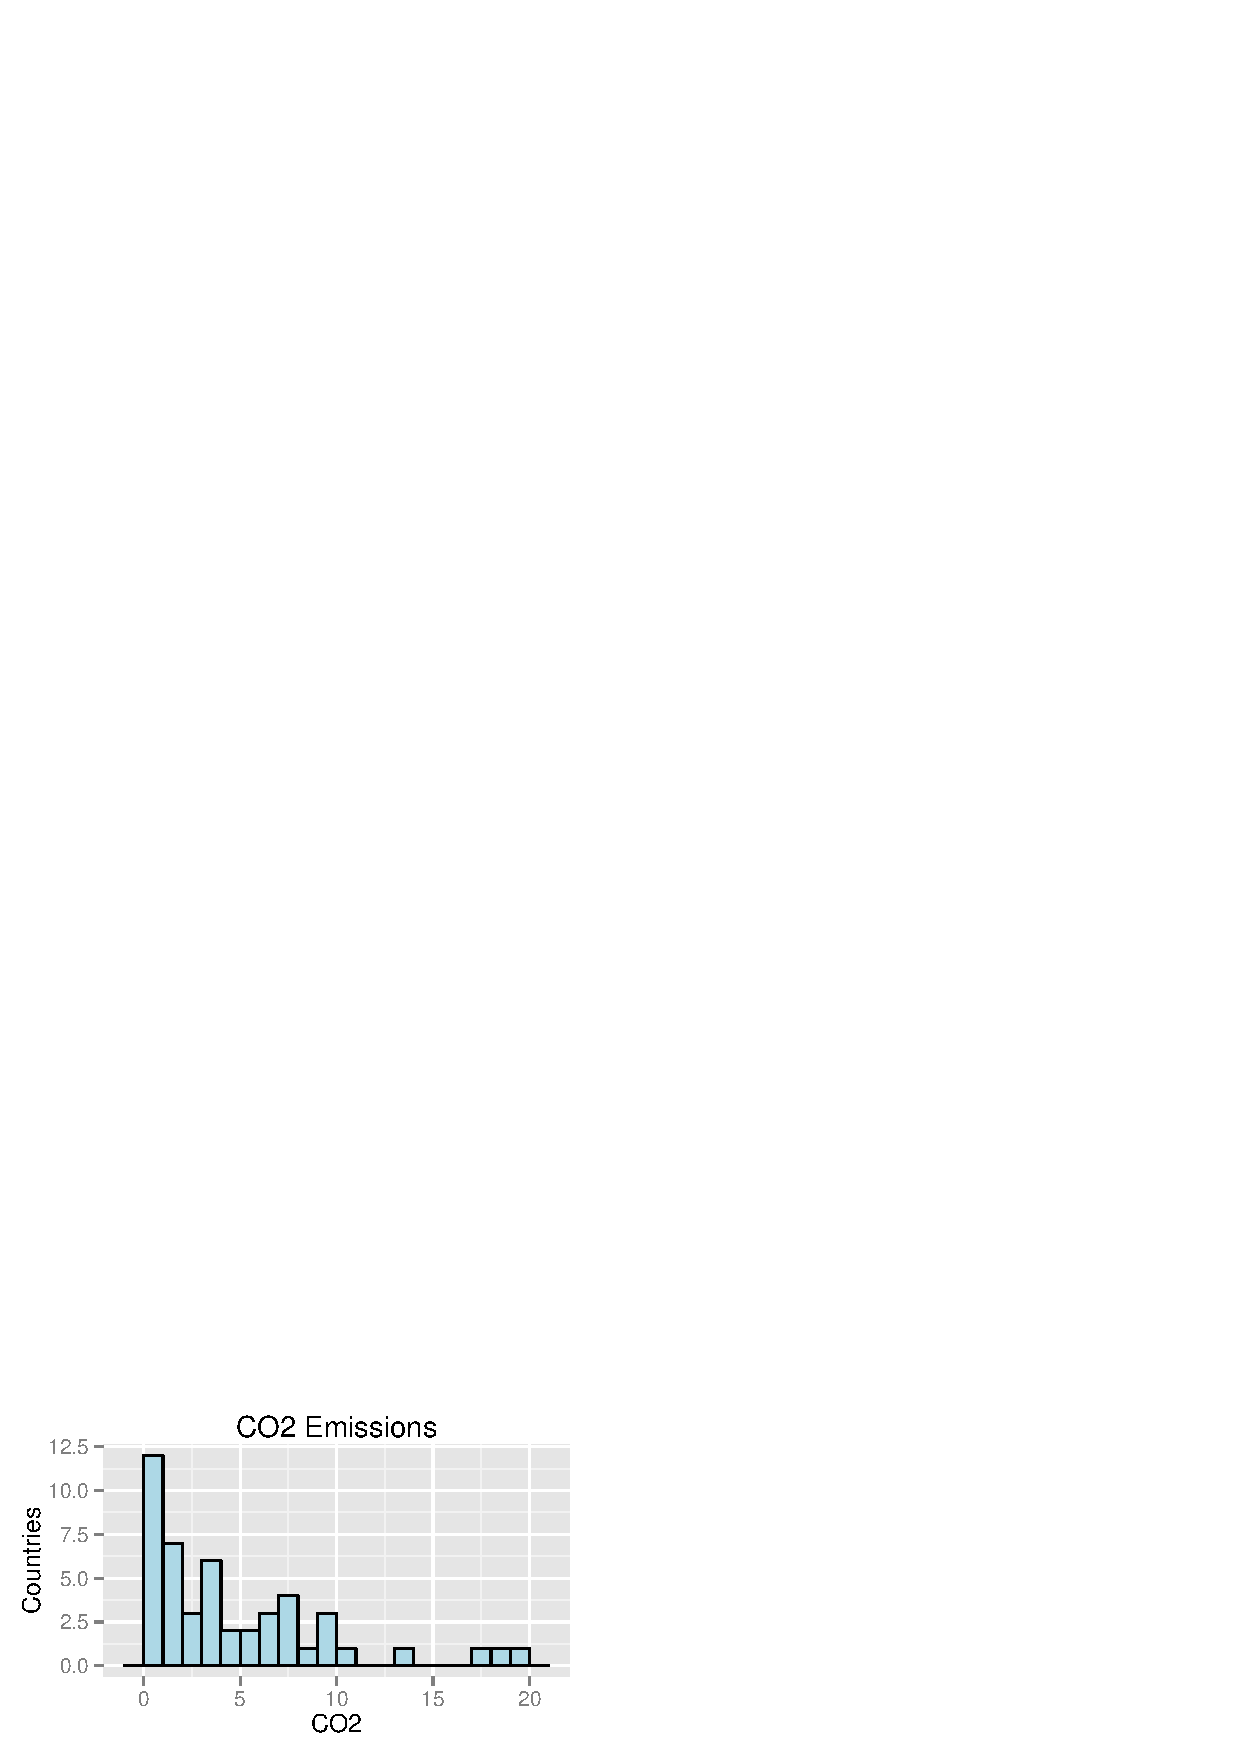
\includegraphics{ex50.pdf}
          \caption{Exercise 50}\label{fig:ex50}
        \end{figure}

        \begin{enumerate}[(a)]
          \item See Figure~\ref{fig:ex50}. The data actually looks left-skewed
            and not particularly normal.

          \item
            \begin{align*}
              \bar{x}     & = \num{30 841} \\
              s_{\bar{x}} & = \frac{3000}{\sqrt{20}} \approx 670.82 \\
              z_{0.95}    & = 1.6445 \\
              \\
              \mu & = 30,841 \pm 1.6445 \cdot 670.82 \\
                  & = \boxed{ \unit[\num{ 30 841 } \pm 1103]{lb} } \\
            \end{align*}

            The 90\% confidence interval is from \fbox{ 29,734 to 31,944 lbs }.
        \end{enumerate}

      \item[51]
        \begin{figure}[ht]
          \centering
          \includegraphics{ex51.pdf}
          \caption{Exercise 51}\label{fig:ex51}
        \end{figure}

        \begin{enumerate}[(a)]
          \item See Figure~\ref{fig:ex51}. 

          \item
            \begin{align*}
              \bar{x} & = -3.587 \\
              s       & = \frac{2.5}{\sqrt{47}} \\
                      & \approx 0.3647 \\
              \\
              z_{0.995} & = 2.5758 \\
              \\
              \mu & = -3.587 \pm 2.5758 \cdot 0.3657 \\
                  & = -3.587 \pm 0.9393 \\
            \end{align*}

            We can be 99\% confident that the average bone loss for the
            population is between $-4.5265$ and $-2.6479$.

        \end{enumerate}

      \item[52]
        From exercise 50:
        \begin{align*}
          \bar{x}          & = 30,841 \\
          \sigma_{\bar{x}} & \approx 670.82 \\
        \end{align*}

        \begin{enumerate}[(a)]

          \item 
            \noindent
            \begin{itemize*}
              \item $H_0$: $\mu = \unit[\num{ 32 000 }]{lb}$
              \item $H_a$: $\mu \ne \unit[\num{ 32 000 }]{lb}$
            \end{itemize*}

            \[
              z = \frac{30,841 - 32,000}{670.82} \approx -1.7277 \\
            \]

            From Table A, if the actual mean is 32,000 lbs, there is a 0.042
            probability of observing a value as small as 30,841 lbs or as large
            as 33,159 (same distance in the other direction).

            The P-value is 0.084 so we can reject the null hypothesis at a
            significance level of 0.10. There is less than a 10\% chance of
            getting a value at least 1159 lbs from 32,000 lbs.

          \item 
            \noindent
            \begin{itemize*}
              \item $H_0$: $\mu = \unit[\num{ 31 500 }]{lb}$
              \item $H_a$: $\mu \ne \unit[\num{ 31 500 }]{lb}$
            \end{itemize*}
            \[
              z = \frac{\num{ 30 841 } - \num{ 31 500 }}{670.82} \approx -0.9824 \\
            \]

            From Table A, if the actual mean is 31,500 lbs, there is a 0.1630
            probability of observing a value of 30,841 or less.

            The two-sided P-value is 0.32 so we can't reject this null hypothesis
            at a significance level of 0.10. If the actual mean is 31,500 lbs,
            there is a 32\% chance of getting a value at least 659 lbs away from
            31,500 lbs with this sample size.

        \end{enumerate}

      \item[53]
        From exercise 51:
        \begin{align*}
            \bar{x}          & = -3.587 \\
            \sigma_{\bar{x}} & \approx 0.3647 \\
        \end{align*}

        \begin{itemize*}
          \item $H_0$: $\mu = 0$
          \item $H_a$: $\mu \ne 0$
        \end{itemize*}

        \[
          z = \frac{-3.587 - 0}{0.3647} \approx -9.8364 \\
        \]

        There is essentially zero chance of getting this result by chance,
        so we can confidently reject the null hypothesis and conclude that
        the moms are losing bone density.

      \newpage

      \item[55]
        \begin{enumerate}[(a)]
          \item 
            \noindent
            \begin{itemize*}
              \item $H_0$: $\mu = 0$
              \item $H_a$: $\mu > 0$
            \end{itemize*}

          \item
            \begin{align*}
              \bar{x} & = 0.10125 \\
              \sigma  & = 0.22 \\
              \mu_0   & = 0 \\
              \\
              s       & = \frac{0.10125}{\sqrt{16}} \approx 0.055 \\
              \\
              z & = \frac{0.10125 - 0}{0.055} \approx 1.8409 \\
            \end{align*}

            From Table A, there is a 0.0328 probability of a value at least this
            high so we can reject the null hypothesis with a P-value of 0.0328.

        \end{enumerate}

      \newpage

      \item[57]
        \begin{enumerate}[(a)]
          \item 
            \begin{align*}
              \bar{x} & = 126.07 \\
              n       & = 72 \\
              \sigma  & = 15 \\
              \\
              \sigma_{\bar{x}} & = \frac{15}{\sqrt{72}} \\
                               & \approx 1.7678 \\
            \end{align*}

            For 95\% confidence:
            \begin{align*}
              \mu & \approx 126 \pm 1.6449 \cdot 1.7678 \\
                  & = 126 \pm 2.9 \\
            \end{align*}

            \fbox{ 123.1 to 128.9 }

          \item 
            \begin{align*}
              z & = \frac{126.07 - 128}{1.7678} \\
                & \approx -1.0918 \\
            \end{align*}

            The p-value is 0.2749

          \item 
            \begin{align*}
              z & = \frac{126.07 - 129}{1.7678} \\
                & \approx -1.6574 \\
            \end{align*}

            The p-value is 0.0974 

        \end{enumerate}

  \end{description}

  \else
    \vspace{10 cm}
    \begin{quote}
      \begin{em}
        And I think that's really something that we all have to remember, is
        that there are cases---and there have been throughout history, and there
        will continue to be throughout time---where what is lawful is not
        necessarily right or necessarily moral. It doesn't take long for an
        American to think back to periods when things were legal but they
        weren't echical, when they weren't moral. And I think today when we see
        similar policies, every citizen has a duty to resist those and to try to
        build a better, more fair society.
      \end{em}
    \end{quote}
    \hspace{1 cm}--Edward Snowden
  \fi

\end{document}

